
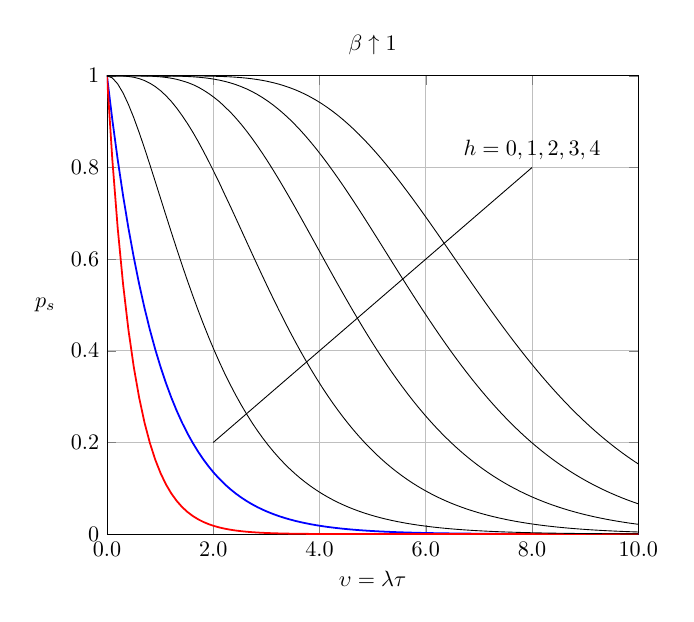
\begin{tikzpicture}[scale=0.8]

\begin{axis}
[
  title={$\beta\uparrow 1$},
%   width  = 0.8*\columnwidth, 
%   height = 0.4*\columnwidth,
  legend style={at={(0.95,0.95)}, anchor=north east},
%   xmode=log,
  xlabel={$\upsilon=\lambda\tau$},
  ylabel={$p_s$}, ylabel style={rotate=-90},
%  yticklabel=\pgfmathprintnumber{\tick}\\ \%,
  xmin = 0, 	
  xmax = 10,
  ymin = 0, 	
  ymax = 1,
  x tick label style={
        /pgf/number format/.cd,
        fixed,
        fixed zerofill,
        precision=1,
        /tikz/.cd
  },
  grid = both,
  scale only axis,
]
% 	\legend{slotted ALOHA, unslotted ALOHA}
    
    \addplot[thick, blue, domain = 0:10, samples=100] {exp(-x)};
    \addplot[thick, red, domain = 0:10, samples=100] {exp(-2*x)};
    
    \addplot[domain = 0:10, samples=100] {(1+x)*exp(-x)};
    \addplot[domain = 0:10, samples=100] {1-((1-exp(-x))^2-x^2*exp(-x))};
    \addplot[domain = 0:10, samples=100] {1-( (1-(1+x)*exp(-x))^2+(1-x-exp(-x))*x^2/2*exp(-x) )};
    \addplot[domain = 0:10, samples=100] {exp(-2*x)/12*(-12-24*x-24*x^2-8*x^3-x^4+2*exp(x)*(12+12*x+6*x^2-2*x^3+x^4))};
    \addplot[domain = 0:10, samples=100] {exp(-2*x)/144*(-144-288*x-288*x^2-192*x^3-66*x^4-12*x^5-x^6+6*exp(x)*( 48+48*x+24*x^2+8*x^3-3*x^4+x^5 ))};
    % \addplot[domain = 0.5:1.04, dashed, samples=100] {x*(1+((-3 + 2*x + sqrt(5 + 4*(-1 + x)*x))/(2*x))*x)*exp(-(2-((-3 + 2*x + sqrt(5 + 4*(-1 + x)*x))/(2*x)))*x)};
    
%     \addplot[thick] table
%     [
% 		x expr = \thisrow{lam},
%     	y expr = \thisrow{25dB}
%     ] {./Data/envelopes.dat};

    \draw[-\arrowhead] (axis cs: 2,0.2) -- (axis cs: 8,0.8) node[anchor=south] 
        {$h =0,1,2,3,4$};
\end{axis}

\end{tikzpicture}
